31. $y=\cfrac{x-2}{|x^2-2x|}=\cfrac{x-2}{|x||x-2|}=\begin{cases} \cfrac{1}{x},\ x>2,\\ -\cfrac{1}{x},\ 0<x<2,\\ \cfrac{1}{x},\ x<0. \end{cases}$
$$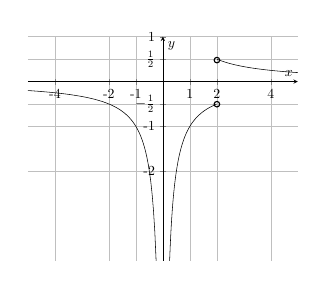
\begin{tikzpicture}[scale=0.5]
\begin{axis}[
    axis lines = middle,
    grid=major,
    legend pos={south west},
    xlabel = {$x$},
    %xlabel style={below right},
    ylabel = {$y$},
    ymin=-4,
    ymax=1,
    xtick={-4, -2,-1,1, 2,4},
    xticklabels={-4, -2,-1, 1, 2, 4},
    ytick={-2,-1,-0.5,0.5, 1, 2},
     yticklabels={-2,-1,$-\frac{1}{2}$,$\frac{1}{2}$, 1, 2},
                  ]
	\addplot[domain=-5:-0.1, samples=100, color=black] {1/x};
    \addplot[domain=0.1:1.99, samples=100, color=black] {-1/x};
    \addplot[domain=2.01:5, samples=100, color=black] {1/x};
   % \addplot[domain=1.01:5, samples=100, color=black] {3/(x+1)};
    %\addlegendentry{$\text{Рис. 1}$};
\end{axis}
\draw (4.8,5.1) circle (2pt);
\draw (4.8,3.98) circle (2pt);
\end{tikzpicture}$$
